\chapter {Network Architecture}

Since the task of image segmentation is a popular one, a number of architecture propositions have been made that aim to produce segmentations. Among them is the \textit{U-Net}, which is the basis of the network used in this thesis.  In the following sections, the principles behind so-called \textit{Convolutional Neural Networks}, the differences between them and normal MLPs and the operations in such networks are detailed.


	\section{Convolutional Neural Networks}
Convolutional Neural Networks (CNNs) are a special subtype of ANNs/MLPs that was popularized by LeCun \cite{lecun98} and, more recently, the successes of Krizhevsky \cite{krizhevsky2012} in the domain of image classification, although CNNs have been applied to other problems such as sound analysis as well. The rationale for their creation was that using fully-connected networks like the ones presented in section \ref{subsec:mlp_backprop} relate all elements of an input vector to every other element, which is generally a good thing to do - however, it ignores the relationship between parts of the input that is given in some datasets and doesn't scale well for very large datasets because of the large number of weights needed. Especially in image data, pixels that are close to each other by some metric such as the Euclidean distance are much more likely to be related, while pixels that lie on the other side of the image hardly are relevant in the context of operations like pixel classification. Consequently, CNNs encode this spatial relationship by using convolution operations (see section \ref{sec:canny}). Concretely, a convolution layer in a CNN typically consists of three sub-components:\\

\noindent First, the data is convoluted by applying one or multiple kernels (also called filter) to all input values and their local neighborhoods.\footnote{Although the convolution in section \ref{sec:canny} describes out-of-bounds handling, the architecture used in this thesis uses only the naturally valid part of the convolution, i.e. if a $3 \times 3 \times d$ filter is used, a 1-value border of the data is lost because the local neighborhood would be partly out of bounds for these border values.} Kernels typically have a size of $k \times k \times d$, where $k$ is the filter size and $d$ is the depth of the dataset, e.g. in an RGB image dataset, the depth is 3 because there are 3 color channels. The result of these convolutions are as many outputs, called \textit{feature maps}, as there are filters in the layer. When viewed as a graph, this means that the hidden neurons represent the results of each convolution step, while all hidden neurons of the same filter share the same weights.

Effectively, this means that the same kind of pattern is searched in the entire dataset, resulting in \textit{translation invariance}, i.e. it doesn't matter where the pattern is because it is still the same pattern at every position in the data.

Then, the feature maps are passed through an non-linear activation function $h(\cdot)$, just like in normal MLPs, to generate activation maps.

\noindent Finally, these activation maps are exposed to a pooling operation such as \textit{Maximum Pooling}. Maximum pooling is a downsampling method that reduces the complexity of the network by replacing groups of values that are apart by a certain stride in the activation map with the maximum value within that group, resulting in a condensed activation map, while performing this calculation for each depth slice of the data independently. Intuitively, some of the information about where a pattern was detected by a filter while creating the feature map is given up in order to make the network easier to train, although the relative positions between patterns are kept intact. \cite[pp. 330-345]{deeplearning_book}\\

\noindent The training of such a network then proceeds like in an MLP, only that the weights that the network has to learn by backpropating the loss through the network are the weights of fully-connected layer as well as the filter weights.\\

\noindent See figure \ref{fig:convnet} for an example of a simple CNN architecture.

\begin {figure}[!ht]
	\begin{center}
		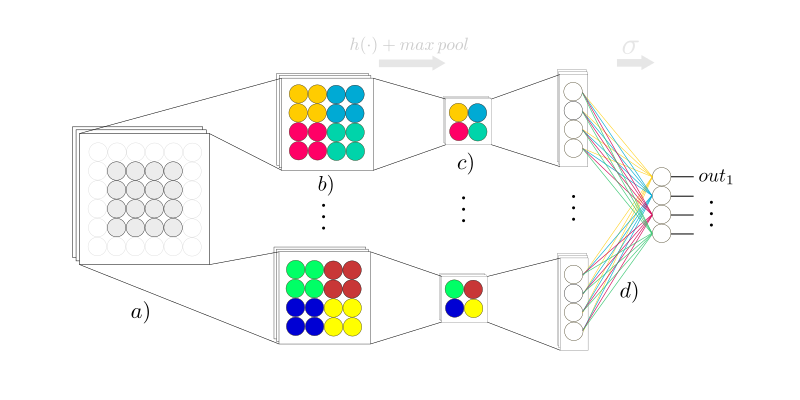
\includegraphics[scale=0.75]{img/fig_convnet}
	\end{center}
	\caption{A Convolutional Neural Network with multiple filters. For simplicity, most neuron connections aren't shown explicitly. \textbf{a):} Input layer. The input size is $6 \times 6 \times 3$, while the kernel size is $3 \times 3 \times 3$. Neurons with valid convolution neighborhoods shown in gray. \textbf{b):} Feature maps with size $4 \times 4 \times 3$ that are the result of applying convolution filters to the input, which are then passed into the activation function $h$ to create activation maps. \textbf{c):} Results of a Maximum Pooling operation with sizes $2 \times 2$ and stride $2$ applied to the activation maps. The colors indicate the downsampled position of the maximum activation in a pooling region. \textbf{d):} Fully-connected output layer that calculates the network outputs via applying the output function $\sigma$. The max-pooled values have been rearranged into a column for clarity, and connections are color-coded by the receiving neuron.}
	\label{fig:convnet}
\end {figure}


	\section {Output- and Loss Functions}

	\subsection{Softmax}
\label{subsec:softmax}

\textit{Softmax} is a function that is usually employed to convert a vector of numbers into probabilities. For example, it can be used as the output function $\sigma$ to transform network scores. The Softmax function for some input vector $z$ is defined as

\[\sigma(z) = \frac{e^{z}}{\sum_{k=0}^{K} e^{z_k}},\]

\noindent where $e$ is the exponential function and $z$ has a dimension of $1 \times K$. The Softmax function acts as a normalizer that ``squashes'' the values of its input vector into the range $[0, 1]$ with respect to relative differences between the vector values. For example, let $z = [-2.432, 1.832, 0.299]$. Then $\sigma(z) = [0.011, 0.813, 0.176]$ is the softmax output for $z$.

These processed values can then be interpreted as probabilities much more naturally than the raw input. However, the above definition of the Softmax function can become numerically unstable when the exponentiation yields large values because dividing by large numbers could potentially produce zero values. To prevent this, it can be made robust by defining it as

\begin {align}
	&z' = z - \max \limits_{i = 0}(0, z_i)\\
	&\sigma(z') = \frac{e^{z'}}{\sum_{k=0}^{K} e^{z'_{{k}}}}
\end {align}


		\subsection{Cross-Entropy Loss}
\label{subsec:cross_ent}

A common loss layer in MLPs that perform multi-class classification is the \textit{Cross-Entropy Loss} layer. In many frameworks, the layer's implementation actually consists of two steps:

First, the input $z$ of the layer is transformed by the softmax function, and then sent to the appended loss function, in which the actual loss computation is done. The \textit{Cross-Entropy Loss} function compares a true probability distribution $p$ to a model probability distribution $q$. For a vector of calculated softmax probabilities $z_i$, it is defined as follows:

\[CE(p, q) = -\sum \limits_{i = 0}^{K} p(i) \log q(i)\]

\noindent Conveniently, the softmax function forces all input values to be positive, allowing the logarithm in the loss to be used. Even though $\log (0)$ isn't defined, the softmax function should never produce values that are exactly equal to zero or one. \textbf{TODO: WHY?} 

\noindent Since each pixel of the input image belongs to one class only, this means that for a given pixel, the probability of its ground truth label is $1.0$, while all others are $0.0$. If, without loss of generality, the third class is assumed to be the ground-truth class, $p$ will be $[0.0, 0.0, 1.0, 0.0]$.  Hence, only the predicted probability of the true third class influences the loss, and all the other summands can be omitted, yielding the condensed general formula

\[CE'(q) = - \log(q_{true}),\]

\noindent where $q_{true}$ denotes the predicted probability for the true class. The loss of the entire image is then calculated as the sum of the losses of all pixels divided by the number of pixels.


		\subsection{Weighted Cross-Entropy Loss}

Using a softmax loss function assumes that all pixels in each training sample should carry the same weight in the backpropagation process. As long as the distribution of classification classes is balanced, this works well, but if it is not, classes with lower probability are trained much more slowly.

To combat this problem, one can introduce a pixelwise weight map for each training sample whose values depend on the ground truth class and the position of each pixel. For example, the softmax loss is changed to

\[CE(p, q) = -\sum \limits_{i = 0}^{K} p(i) \log q(i) \cdot w(i),\]

\noindent where $w(i)$ is the weight for pixel $i$.

 The weight for each pixel is calculated as follows:

\[ w(i) = w_c(i) + w_0 \cdot \exp \left (- \frac{(d_1(i) + d_2(i))^2}{2\sigma^2} \right ), \]

\noindent where $w_c$ is the class-specific weight for the pixel's ground truth class, $d_1$ and $d_2$ are the euclidean distances to the nearest and second-nearest non-background pixel and $w_0$ and $\sigma$ are additional modifier terms. 


		\subsection{F-Measure}

An alternative to solving the problem of unbalanced classes in the training data is using the F-Measure, also called DICE similarity or $F_1$-Score, as a loss function instead. The F-Measure is a statistical similarity function which has been shown to perform well on unbalanced data\cite{fmeasure1}\cite{fmeasure2}\cite{fmeasure3} defined as

\[F_1 = 2 \cdot \frac{PR \cdot RC}{PR + RC},\]

\noindent where PR denotes the \textit{Precision} and RC denotes the \textit{Recall} over the training sample in comparison to its ground truth. In turn, \textit{Precision} is defined as

\[PR = \frac{TP}{TP + FP}\]

\noindent and \textit{Recall} is defined as

\[RC = \frac{TP}{TP + FN},\]

\noindent where TP is the number of true positives, FP is the number of false positives, and FN is the number of false negatives. \textbf{TODO}: Wie kann man FP etc auf ein Mehrklassen-Problem anwenden?

	\section {The U-Net Architecture}
The U-Net is a CNN architecture proposed by Ronneberger et al.\cite{unet} which aims to produce segmentation maps for images of cells. It was implemented using Caffe\cite{caffe}, a CNN library developed by the University of California, Berkeley that allows CNN layers - such as the ones described in the previous section - to be put together to form a network.

% Image of U-Net here 
